\clearpage
\chapter*{PHỤ LỤC}
\phantomsection
\addcontentsline{toc}{chapter}{PHỤ LỤC}
\setcounter{table}{0}
\renewcommand{\thetable}{A.\arabic{table}}

\section*{A - BẢNG PHÂN CÔNG CÔNG VIỆC}
\phantomsection
\addcontentsline{toc}{section}{A - BẢNG PHÂN CÔNG CÔNG VIỆC}

\begin{table}[H]
\centering
\caption{Phân công công việc và tỷ lệ đóng góp của thành viên}
\label{tab:team_contributions}
\begingroup
\setlength{\tabcolsep}{3pt}
\renewcommand{\arraystretch}{1.12}
\begin{tabularx}{\textwidth}{|P{1.0cm}|P{4.7cm}|P{4.0cm}|>{\centering\arraybackslash}X|}\hline
\textbf{Mã} & \textbf{Thành viên} & \textbf{Vai trò} & \textbf{\% đóng góp} \\\hline
TV1 & Nguyễn Hoàng Anh & Leader, DBSCAN nền tảng và tích hợp & 100\% \\\hline
TV2 & Lý Huỳnh Phương Anh & Lý thuyết Incremental DBSCAN và INSERT & 100\% \\\hline
TV3 & Từ Thiên Gia Bảo & Thiết kế OOP, DBSCAN và DELETE & 100\% \\\hline
TV4 & Nguyễn Phạm Gia Bảo & Dữ liệu, thực nghiệm và trực quan hóa & 100\% \\\hline
TV5 & Hồ Ngọc Bảo & Không tham gia đồ án & 0\% \\\hline
\end{tabularx}
\endgroup
\end{table}

\section*{B - CÔNG BỐ VIỆC SỬ DỤNG AI}
\phantomsection
\addcontentsline{toc}{section}{B - CÔNG BỐ VIỆC SỬ DỤNG AI}

Trong quá trình thực hiện đồ án, nhóm có sử dụng ChatGPT/Codex như công cụ hỗ trợ. Công cụ được dùng để đề xuất và chỉnh sửa một số đoạn mã, giải thích tài liệu thuật toán, biên tập nội dung báo cáo và hỗ trợ định dạng LaTeX.

AI không được dùng để thay thế các phép chạy thực nghiệm hoặc tạo ra các con số kết quả trình bày trong báo cáo. Các số liệu được lấy từ chương trình, notebook và các file kết quả trong repository. Nhóm chịu trách nhiệm kiểm tra mã nguồn, đối chiếu cách cài đặt với tài liệu tham khảo, xem lại kết quả chạy và chỉnh sửa nội dung trước khi nộp.

\section*{C - MÃ NGUỒN VÀ HƯỚNG DẪN CHẠY}
\phantomsection
\addcontentsline{toc}{section}{C - MÃ NGUỒN VÀ HƯỚNG DẪN CHẠY}

Mã nguồn và dữ liệu của đề tài được lưu trong repository của nhóm: \href{https://github.com/hoanganh-kevz/INCREMENTAL_DBSCAN_NHOM_1}{Incremental DBSCAN Nhóm 1}. Các lệnh dưới đây được chạy từ thư mục gốc repository.

Trang thống kê người đóng góp của repository được xem tại \href{https://github.com/hoanganh-kevz/INCREMENTAL_DBSCAN_NHOM_1/graphs/contributors?from=1\%2F8\%2F2026}{GitHub Contributors}.

\begin{enumerate}
    \item Tạo môi trường Python và cài thư viện:
\begin{verbatim}
python -m venv .venv
.venv\Scripts\Activate.ps1
python -m pip install -r requirements.txt
\end{verbatim}
    \item Chạy demo ngắn INSERT/DELETE:
\begin{verbatim}
python run_demo.py
\end{verbatim}
    \item Mở notebook minh họa thuật toán và notebook so sánh:
\begin{verbatim}
jupyter notebook notebooks/Incremental_DBSCAN_Demo.ipynb
jupyter notebook notebooks/So_sanh_thuat_toan.ipynb
\end{verbatim}
    \item Chạy đối chiếu và kiểm tra tự động khi cần:
\begin{verbatim}
python -m src.evaluation.equivalence
python -m pytest tests/
\end{verbatim}
\end{enumerate}

\begin{itemize}
    \item Mã thuật toán: \path{src/clustering/}.
    \item Silhouette tự cài: \path{src/evaluation/metrics.py}.
    \item Dữ liệu demo: \path{data/raw/}.
    \item Các phương pháp scikit-learn dùng làm đối chứng: \path{baseline/}.
\end{itemize}

\section*{D - KẾT QUẢ, HÌNH ẢNH BỔ SUNG}
\phantomsection
\addcontentsline{toc}{section}{D - KẾT QUẢ, HÌNH ẢNH BỔ SUNG}
\setcounter{figure}{0}
\renewcommand{\thefigure}{D.\arabic{figure}}

Hình~\ref{fig:appendix_edge_gallery} tập hợp một số tình huống biên dùng để quan sát điểm đúng trên ngưỡng Eps, điểm chuyển trạng thái và các dạng cập nhật phức tạp hơn. Hình~\ref{fig:appendix_scaling} minh họa sự khác nhau về thang đo thuộc tính trước và sau chuẩn hóa trên luồng thẻ.

\begin{figure}[H]
\centering
    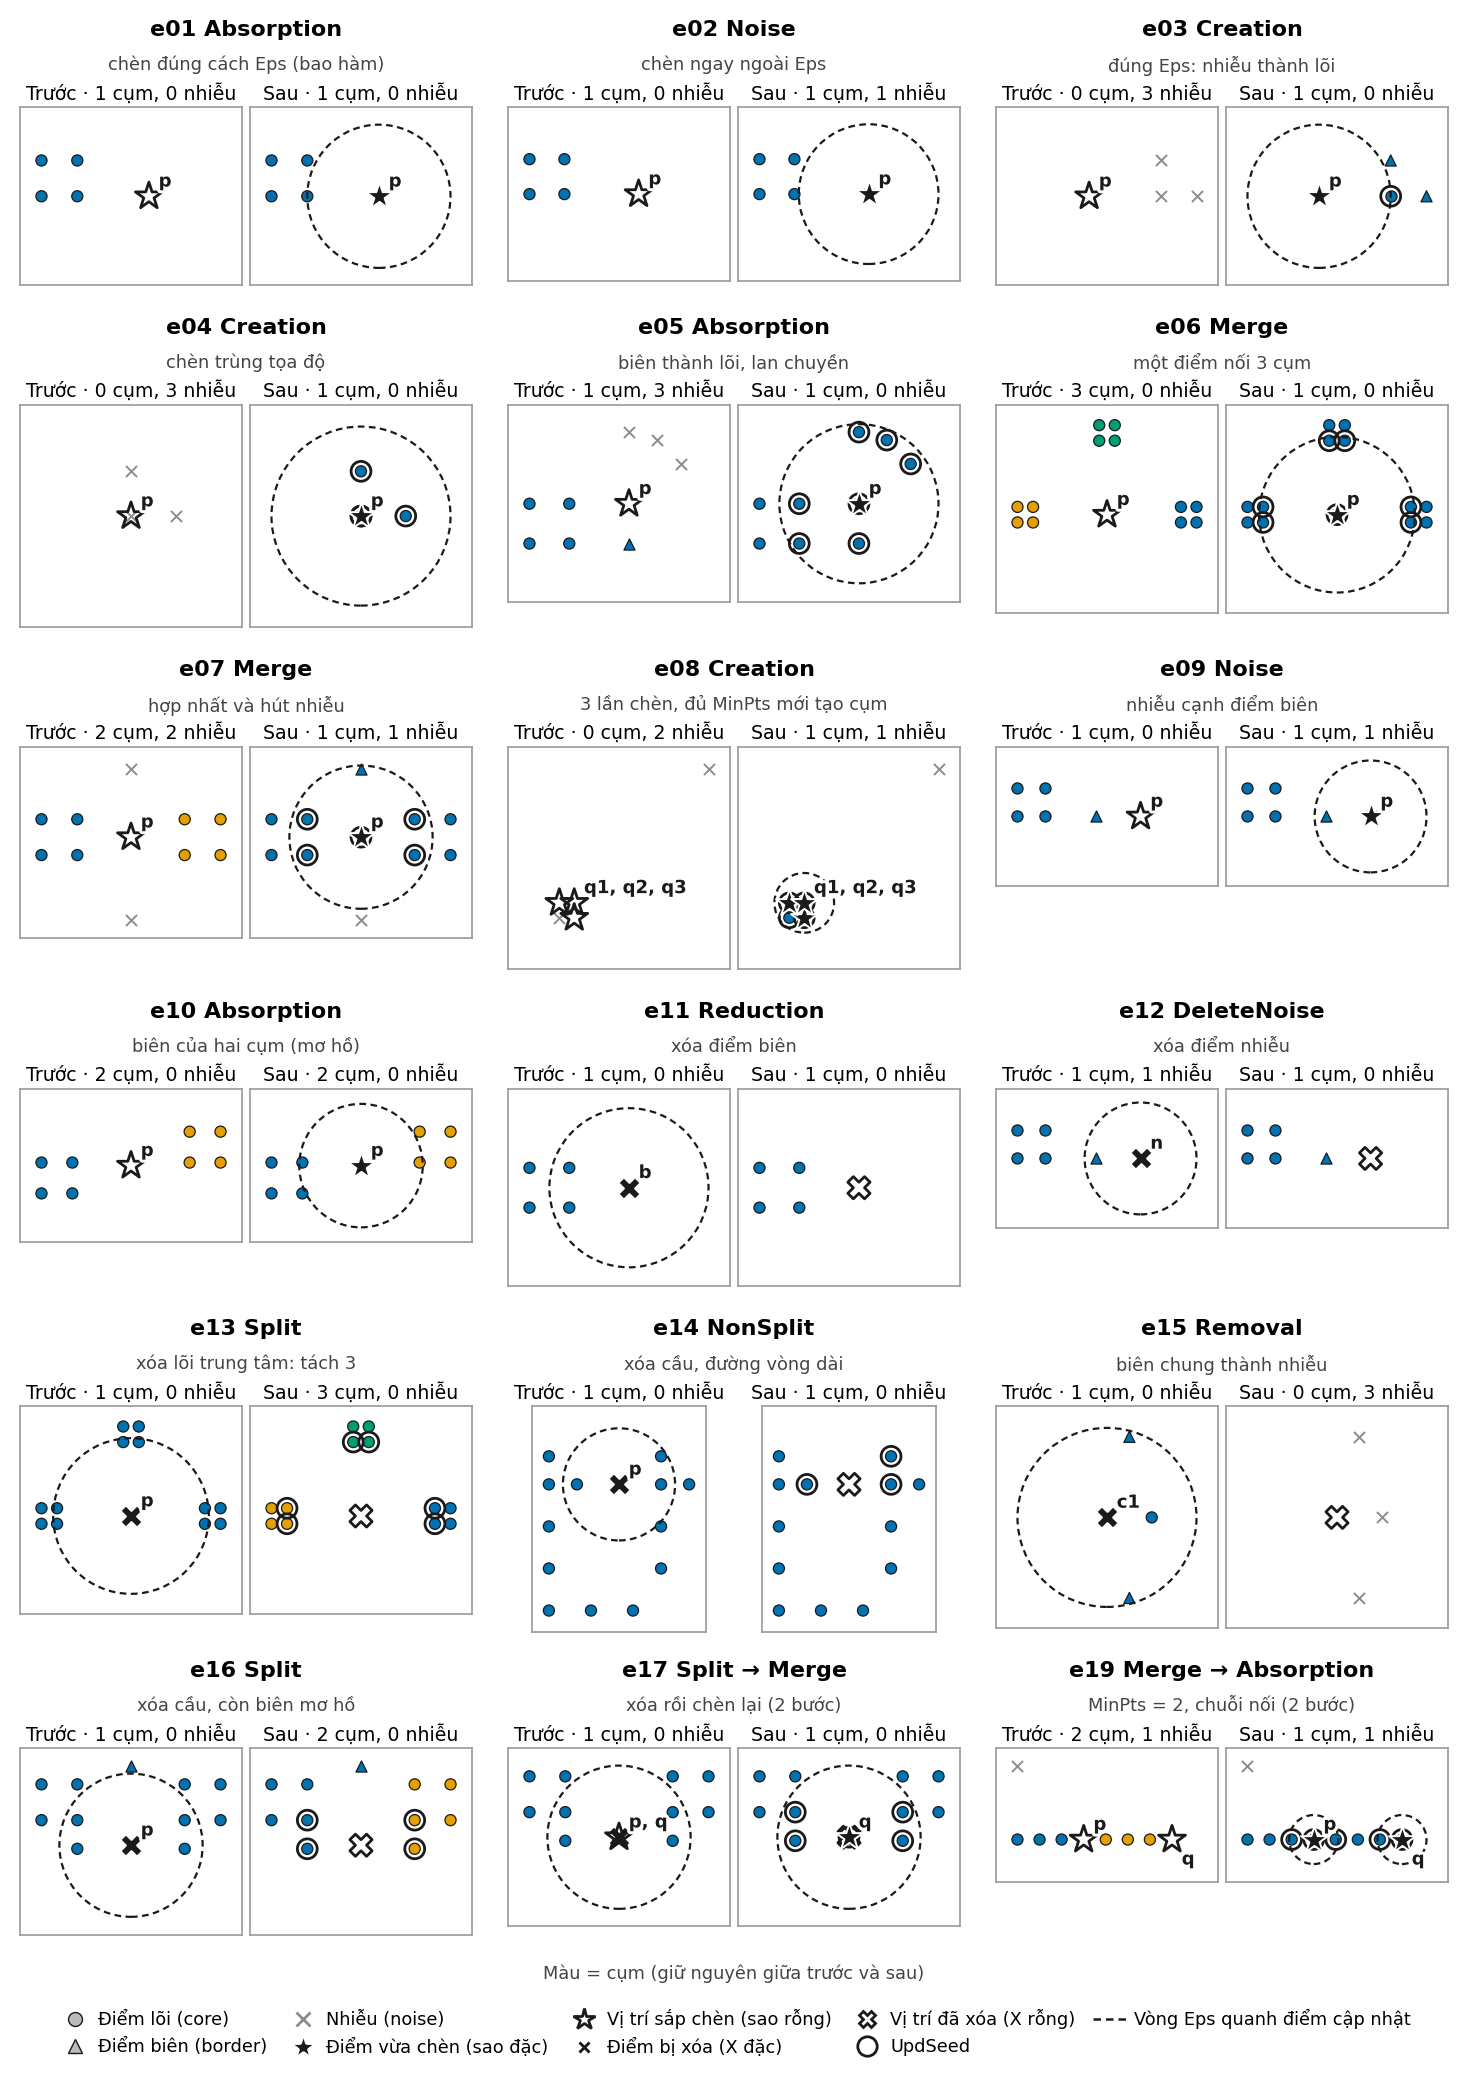
\includegraphics[width=\textwidth,height=0.72\textheight,keepaspectratio]{Images/case_gallery_edge.png}
\caption{Một số trường hợp biên bổ sung của thao tác thêm và xóa điểm}
\label{fig:appendix_edge_gallery}
\end{figure}

\begin{figure}[H]
\centering
    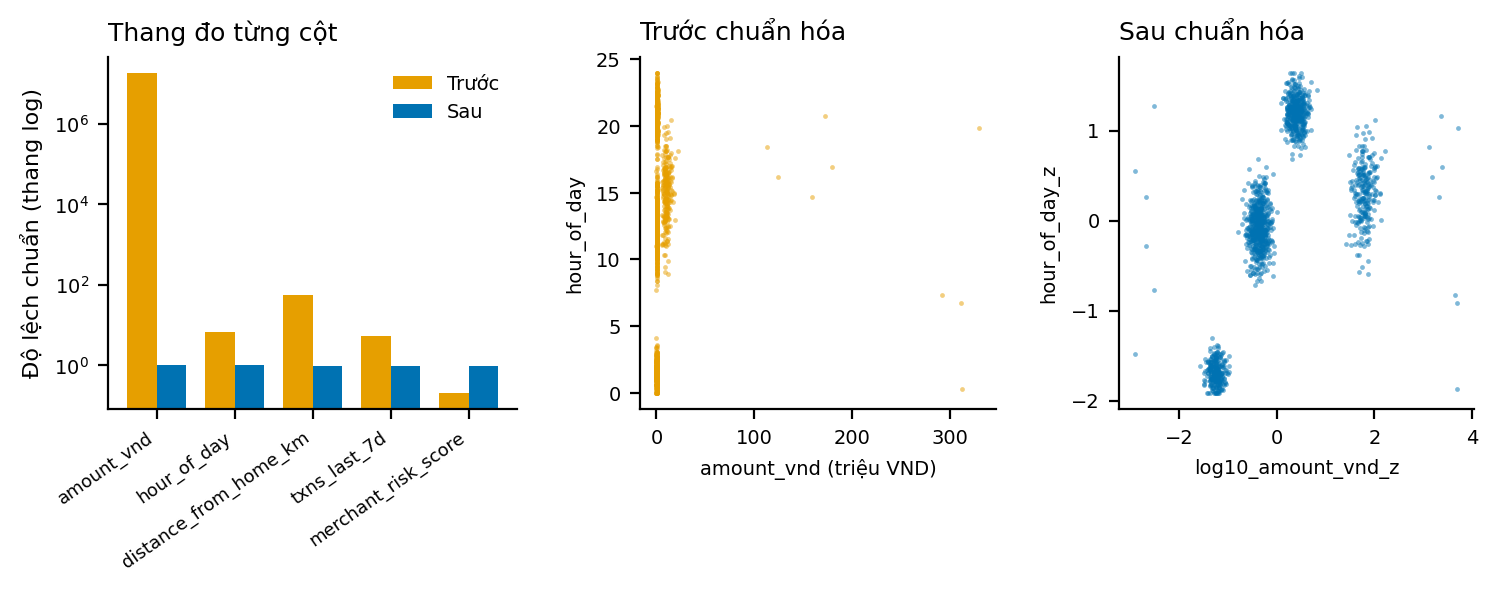
\includegraphics[width=\textwidth]{Images/scaling_effect_card.png}
\caption{Thang đo đặc trưng luồng thẻ trước và sau chuẩn hóa}
\label{fig:appendix_scaling}
\end{figure}
